\subsection{Code example}

In this section, we introduce the reader to a simple example program of Jolie module system to a sophisticated design pattern \textit{Service Injection Pattern}, which is a dependency-injection like design pattern made possible from the implementation of the module system.

The following code snippet is a hello-world example of the Jolie module system.

\begin{listing}[H]
    \lstset{language=Jolie,
        style=codeStyle,
        numbers=left,
        firstnumber=1
    }
    \begin{lstlisting}[frame=tlrb,
basicstyle=\footnotesize]{service-hello.ol}
from console import ConsoleService, ConsoleInterface

service main(){

    outputPort Console {
        interfaces: ConsoleInterface
    }

    embed ConsoleService() in Console

    main{
        print@Console("Hello")()
    }
}
\end{lstlisting}

\end{listing}

At line 1, we declared an import statement to include the ConsoleService along with the interface exposed by this service. The ConsoleService is a build-in service that allows a Jolie program to communicate to the execution process's system console. Afterward, we declare a service node called \textit{main}, which consists of an output port with an assignment of operations in the ConsoleInterface binding to the embed service of the ConsoleService, and the main procedure of the service. 
In our main procedure, we send an operation \textit{print} through the output port Console. Executing this program resulted in Hello is printed on the process console.

\subsubsection{Service Injection Pattern}

Our last example describes a way to compose a simple service in the Jolie module system. Here we can extend the previous example to an advanced scenario. Given a situation where we want to have our workflow on the operation \textit{print}, the developer can create a new service, \textit{PrinterService}, which exposes the operation \textit{print} and prefixing an incoming message before forwarding it to the system console.

\begin{listing}[H]
    \lstset{language=Jolie,
        style=codeStyle,
        numbers=left,
        firstnumber=1
    }
    \begin{lstlisting}[frame=tlrb,
basicstyle=\footnotesize]{printer.ol}

from console import ConsoleService, ConsoleInterface

interface PrinterInterface {
RequestResponse:
    print( undefined )( void )
}

service PrinterService() {

    execution { concurrent }
    
    inputPort IP {
        location: "local"
        interfaces: PrinterInterface
    }

    embed ConsoleService in new _Console

    main{
        [print(req)(res){
            res = "Printer receive: " + req
            print@_Console(res)()
        }]
	// omitted code
    }
}

\end{lstlisting}

\end{listing}

After the service has defined, the developer only has to import and embed \textit{PrinterService} instead of \textit{ConsoleService} in our last example. The client of this service will now point the operation target to the \textit{PrinterService}.

\begin{listing}[H]
    \lstset{language=Jolie,
        style=codeStyle,
        numbers=left,
        firstnumber=1
    }
    \begin{lstlisting}[frame=tlrb,
basicstyle=\footnotesize]{service-injection-hello.ol}
from console import ConsoleInterface
from .printer import PrinterService

service main(){

    outputPort Console {
        interfaces: ConsoleInterface
    }

    embed PrinterService() in Console

    main{
        print@Console("Hello")()
    }
}
\end{lstlisting}
\end{listing}

Since the \textit{PrinterService} operation \textit{print} is defined as a subset of operations in \textit{ConsoleService}. Thus, these two interfaces are compatible to each other.

The module system extends the flexibility of the way we implement a service in Jolie and allows the service developer to create a new system in a modular approach. In the next section, we will look at the practical Jolie module system implementation of the Circuit Breaker, which is one of the prominent  Microservice pattern. 

\subsubsection{Microservice Pattern: Circuit Breaker}
In this section, we discuss an implementation of the circuit breaker pattern in Jolie and emphasize Jolie's capability as a language for microservices. After the discussion on implementation source code, we also explore the integration of this application with the container technology, particularly Docker container.

The circuit breaker is a well-known pattern in the Microservice Architecture. It enables an application to proceed on a request properly on the situation of an arbitrary dependent service that has failed to progress. Given a situation where the network of service communicates with each other to build up the client's response, and one of the services is making a longer than usual processing time. This processing time can be a result of the network latency, or there might be a failure during processing, which cannot foresee by other services. The circuit breaker pattern is a pattern addressing a problem when a dependent service fails to process the request either from the longer than usual processing time or an unexpected error thrown from the invocation. The pattern increases the fault-tolerant of the whole system and helps the service maintainer investigate the issues precisely.

A circuit breaker implementation in the Microservice ecosystem is a proxy between a client to a service that might have failed to deliver the response. The circuit breaker monitors the request and counts the number of failures that happen through calls made to the destination service. If the number of failures reaches the threshold, it discards and returns a meaningful response for the client without attempting to make a call to the destination service. Later after a certain amount of time, on the invocation to the service, the circuit breaker slowly forwards the request again.

There are three states in Circuit breaker which determine the state of calls made to the destination service. Firstly, the \textit{Closed} state is a healthy state of the circuit breaker; at this state, every request for an operation will be passed to the service. Each failure occurred from the call, either internally from the service or the request timeout, the circuit breaker increases the counter. When the number of failures reaches the threshold number, the circuit breaker trips by changes its state to \textit{Open} state and start a reset timeout. At this state, any request making to the destination operation is skipped by the circuit breaker as it is presumed that the destination service is down. The developer of the circuit breaker can design the failback procedure, for example, return a cached response to the client or straightforwardly return an error response. After the reset timeout tick, the circuit breaker changes its state to \textit{Half-Open}, where any call will be passed to the service destination. If the service responds without any error, the circuit breaker sets its state to \textit{Close} or in a healthy state. Otherwise, the circuit breaker falls back to status \textit{Open} again. The states for a circuit status illustrate in the figure ~\ref{list:circuit-breaker}.

\begin{figure}[ht]
    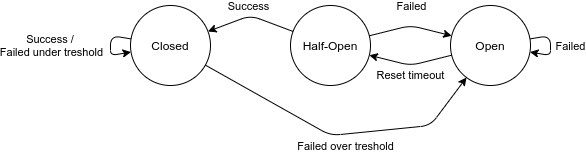
\includegraphics[width=10cm]{CircuitBreaker}
    \centering
    \caption{A state diagram for Circuit Breaker}
    \label{list:circuit-breaker}
\end{figure}

Montesi and Weber have studied the implementation of the circuit breaker pattern for Jolie application\cite{10.1145/3167132.3167427}, which extends a decoration pattern and sketch an implementation of the circuit breaker pattern in Jolie. In our version, we exploit the capability of importing service to extend a single service with a circuit breaker extension service.

Start with a circuit breaker service, which implemented as an extension service to be imported and embedded by others. We firstly define definitions for the circuit breaker. As a requirement above, we define two communication ports to manage the functionality of the service, one for managing the communication between the circuit breaker to the destination service for handling the internal operation such as timeout for resetting the \textit{Opened} state and request timeout handler. Furthermore, we also define a type for configuring the service. As a proxy service, we require additional input from the embedder service, the exposing input location, and the target location. The source code for what we have mentioned so far is show at ~\ref{list:circuit-breaker-skel-application}

The client requests are handled through an HTTP protocol with a special configuration \textit{default}, which will be invoked as a default operation when the undefined operation is passed to the service. It is worth mentioning that we give the authority to importer service to configure \textit{location} of our \textit{HTTPInput} and \textit{DestService} field by assigning the service parameter.


\begin{figure}[ht]
    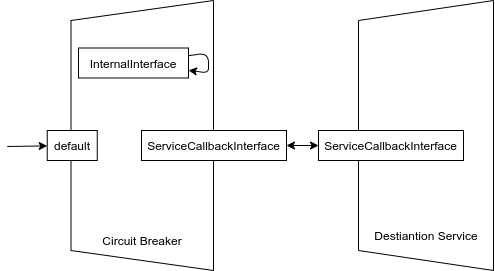
\includegraphics[width=10cm]{CircuitBreakerDiagram}
    \centering
    \caption{A service diagram for Circuit Breaker application}
    \label{list:circuit-breaker-skel-application}
\end{figure}

\begin{listing}[H]
    \lstset{language=Jolie,
        style=codeStyle,
        numbers=left,
        firstnumber=1
    }
    \begin{lstlisting}[frame=tlrb,
basicstyle=\footnotesize]{circuitbreaker-definitions.ol}
interface HTTPInterface{
    requestResponse:
        default(undefined)(undefined)
}

interface CircuitBreakerServiceCallbackInterface{
    requestResponse: callback(undefined)(undefined) throws UnexpectedError(string)
}

type CircuitBreakerServiceParam : void {
    inputLocation: string
    outputLocation: string
}

private interface CircuitBreakerInternalInterface{
    oneWay: reset(undefined)
}

service CircuitBreakerService (p : CircuitBreakerServiceParam) { 
    inputPort HTTPInput {
        protocol: "http" {
            default = "default"
        }
        location: p.inputLocation
        interfaces: HTTPInterface
    }

    outputPort DestService {
        location: p.outputLocation
        protocol: "sodep"
        interfaces: CircuitBreakerServiceCallbackInterface
    }

    inputPort SelfInput{
        location: "local"
        interfaces: CircuitBreakerInternalInterface
    }

    ...

}

\end{lstlisting}
\end{listing}

Next, we define procedures and workflow for each operation exposed by the circuit breaker. The procedures included in this service encapsulate the actions made for state transformation. We use a global state, a shared state lived in every session initiated by the service, to store the counter of error number and the flag of the current status of the circuit breaker.

    \lstset{language=Jolie,
        style=codeStyle,
        breaklines=true,
        columns=fullflexible,
        numbers=left,
        breaklines=true,
        firstnumber=1
    }
    \begin{lstlisting}[frame=tlrb,
basicstyle=\footnotesize]{circuitbreaker-port.ol}
constants {
    STATUS_CLOSED = 1,
    STATUS_OPEN = 2,
    STATUS_HALFOPEN = 3,
    ERROR_THRESHOLD = 3,
    TIMEOUT_REQUEST = 1000
}

service CircuitBreakerService (p : CircuitBreakerServiceParam) {
    ...
    define closeCircuit {
        global.errorCount = 0
        global.status = STATUS_CLOSED
    }

    define resetCircuit {
        global.status = STATUS_HALFOPEN
    }

    define trip {
        global.status = STATUS_OPEN
        scheduleTimeout@Time( TIMEOUT_REQUEST{.operation="reset"} )( )
    }

    define handleError {
        if (global.status == STATUS_HALFOPEN){
            trip
        } else if (global.errorCount > ERROR_THRESHOLD){
            trip
        }
    }

    execution { concurrent }

    init {
        closeCircuit
    }

    main {        
        [ reset() ]{
            resetCircuit
        }
        [ default( request )( response ) {
            if ( global.status == STATUS_OPEN ){
                response = "CircuitOpen"
            } else {
                install( UnexpectedError =>
                    global.errorCount++
                    handleError
                    response = "ServiceError"
                )
                callback@DestService(request)(serviceRes)

                if (global.status == STATUS_HALFOPEN){
                    closeCircuit
                }

                response << serviceRes
            }
        }]
    }
}
\end{lstlisting}

The \textit{trip} procedure defines the instruction set to turn on the circuit, which is determined by procedure \textit{handleError}. After modifying the state, it proceeds with scheduling the timeout request for state recovery, defined in \textit{resetCircuit}, by invoking the operation from build-in service \textit{time} \footnote{Time service specification https://jolielang.gitbook.io/docs/language-tools-and-standard-library/standard-library-api/time}. 

The circuit breaker's initialization begins with a call to procedure \textit{closeCircuit}, which sets the state of the circuit to \textit{Closed} state. Later in the main execution, the service exposes and wait for two operations \textit{reset} and \textit{default}. The \textit{reset} operation is responsible for turn an Opened state of the circuit breaker to \textit{Half-Opened} by calling \textit{resetCircuit} procedure defined above. The operation for handling client requests, \textit{default}, as mention above, is invoked whenever the client is passing a message to the circuit breaker and forward the request to the destination service. The workflow of operation can be described as the following:
If the state of the circuit breaker, return a response without passing the request to destination service.
Otherwise, forward the request to destination service, if there is an error occur, call the error handling procedure and return a response to the client.

After we have defined the CircuitBreaker service, which can be imported and embed by any services, we look into an example service \textit{AddService}, which integrates the CircuitBreaker extension to handle the possible error that might occur internally. 

\begin{listing}[ht]
    \lstset{language=Jolie,
        style=codeStyle,
        numbers=left,
        firstnumber=1
    }
    \begin{lstlisting}[frame=tlrb,
basicstyle=\footnotesize]{circuitbreaker-client.ol}
from .circuitbreaker import CircuitBreakerService, CircuitBreakerServiceCallbackInterface

type input: void{
    x : int
    y : int
}

interface calculatorIface {
    requestResponse: 
        add(input)(int)
}

service main {

    inputPort SelfIn {
        location: "local://self"
        interfaces: calculatorIface
    }

    outputPort SelfOp {
        location: "local://self"
        interfaces: calculatorIface
    }

    inputPort fromCircuitBreaker{
        location: "socket://localhost:3001"
        protocol: "http"
        interfaces: CircuitBreakerServiceCallbackInterface
    }

    embed CircuitBreakerService( { 
        inputLocation = "socket://localhost:3000"
        outputLocation = "socket://localhost:3001" 
    } )

    execution { concurrent }

    main{
        [add(req)(res){
		...
        }]
        [callback(req)(res){
                    if (req.operation == "add"){
                        add@SelfOp({x = int(req.data.x) y = int(req.data.y)})(response)               
                    }       

		    if (error){
	    		throw ( UnexpectedError )
		    }else{
			res << response
         	}                  
            }
        }]
    }
}
\end{lstlisting}
\end{listing}

Our implementation of the circuit breaker embedder ~\ref{circuitbreaker-client.ol} requires defining an operation \textit{callback}, which receives a message from the circuit breaker and redirect the request to proper operation. In this case, the workflow includes checking the request operation from \textit{operation} field then forward the message to an internal input port, defined using \textit{local} scheme for location. After the call is complete, return the corresponding result to the circuit breaker.

We had demonstrated an implementation of the microservice architecture, the circuit breaker, using the new feature of the module system. The Jolie module system enables Jolie developer to create and compose multiple sole responsibility services and create a more complex application using the import mechanism.